% Options for packages loaded elsewhere
\PassOptionsToPackage{unicode}{hyperref}
\PassOptionsToPackage{hyphens}{url}
%
\documentclass[
]{article}
\usepackage{amsmath,amssymb}
\usepackage{iftex}
\ifPDFTeX
  \usepackage[T1]{fontenc}
  \usepackage[utf8]{inputenc}
  \usepackage{textcomp} % provide euro and other symbols
\else % if luatex or xetex
  \usepackage{unicode-math} % this also loads fontspec
  \defaultfontfeatures{Scale=MatchLowercase}
  \defaultfontfeatures[\rmfamily]{Ligatures=TeX,Scale=1}
\fi
\usepackage{lmodern}
\ifPDFTeX\else
  % xetex/luatex font selection
\fi
% Use upquote if available, for straight quotes in verbatim environments
\IfFileExists{upquote.sty}{\usepackage{upquote}}{}
\IfFileExists{microtype.sty}{% use microtype if available
  \usepackage[]{microtype}
  \UseMicrotypeSet[protrusion]{basicmath} % disable protrusion for tt fonts
}{}
\makeatletter
\@ifundefined{KOMAClassName}{% if non-KOMA class
  \IfFileExists{parskip.sty}{%
    \usepackage{parskip}
  }{% else
    \setlength{\parindent}{0pt}
    \setlength{\parskip}{6pt plus 2pt minus 1pt}}
}{% if KOMA class
  \KOMAoptions{parskip=half}}
\makeatother
\usepackage{xcolor}
\usepackage[margin=1in]{geometry}
\usepackage{color}
\usepackage{fancyvrb}
\newcommand{\VerbBar}{|}
\newcommand{\VERB}{\Verb[commandchars=\\\{\}]}
\DefineVerbatimEnvironment{Highlighting}{Verbatim}{commandchars=\\\{\}}
% Add ',fontsize=\small' for more characters per line
\usepackage{framed}
\definecolor{shadecolor}{RGB}{248,248,248}
\newenvironment{Shaded}{\begin{snugshade}}{\end{snugshade}}
\newcommand{\AlertTok}[1]{\textcolor[rgb]{0.94,0.16,0.16}{#1}}
\newcommand{\AnnotationTok}[1]{\textcolor[rgb]{0.56,0.35,0.01}{\textbf{\textit{#1}}}}
\newcommand{\AttributeTok}[1]{\textcolor[rgb]{0.13,0.29,0.53}{#1}}
\newcommand{\BaseNTok}[1]{\textcolor[rgb]{0.00,0.00,0.81}{#1}}
\newcommand{\BuiltInTok}[1]{#1}
\newcommand{\CharTok}[1]{\textcolor[rgb]{0.31,0.60,0.02}{#1}}
\newcommand{\CommentTok}[1]{\textcolor[rgb]{0.56,0.35,0.01}{\textit{#1}}}
\newcommand{\CommentVarTok}[1]{\textcolor[rgb]{0.56,0.35,0.01}{\textbf{\textit{#1}}}}
\newcommand{\ConstantTok}[1]{\textcolor[rgb]{0.56,0.35,0.01}{#1}}
\newcommand{\ControlFlowTok}[1]{\textcolor[rgb]{0.13,0.29,0.53}{\textbf{#1}}}
\newcommand{\DataTypeTok}[1]{\textcolor[rgb]{0.13,0.29,0.53}{#1}}
\newcommand{\DecValTok}[1]{\textcolor[rgb]{0.00,0.00,0.81}{#1}}
\newcommand{\DocumentationTok}[1]{\textcolor[rgb]{0.56,0.35,0.01}{\textbf{\textit{#1}}}}
\newcommand{\ErrorTok}[1]{\textcolor[rgb]{0.64,0.00,0.00}{\textbf{#1}}}
\newcommand{\ExtensionTok}[1]{#1}
\newcommand{\FloatTok}[1]{\textcolor[rgb]{0.00,0.00,0.81}{#1}}
\newcommand{\FunctionTok}[1]{\textcolor[rgb]{0.13,0.29,0.53}{\textbf{#1}}}
\newcommand{\ImportTok}[1]{#1}
\newcommand{\InformationTok}[1]{\textcolor[rgb]{0.56,0.35,0.01}{\textbf{\textit{#1}}}}
\newcommand{\KeywordTok}[1]{\textcolor[rgb]{0.13,0.29,0.53}{\textbf{#1}}}
\newcommand{\NormalTok}[1]{#1}
\newcommand{\OperatorTok}[1]{\textcolor[rgb]{0.81,0.36,0.00}{\textbf{#1}}}
\newcommand{\OtherTok}[1]{\textcolor[rgb]{0.56,0.35,0.01}{#1}}
\newcommand{\PreprocessorTok}[1]{\textcolor[rgb]{0.56,0.35,0.01}{\textit{#1}}}
\newcommand{\RegionMarkerTok}[1]{#1}
\newcommand{\SpecialCharTok}[1]{\textcolor[rgb]{0.81,0.36,0.00}{\textbf{#1}}}
\newcommand{\SpecialStringTok}[1]{\textcolor[rgb]{0.31,0.60,0.02}{#1}}
\newcommand{\StringTok}[1]{\textcolor[rgb]{0.31,0.60,0.02}{#1}}
\newcommand{\VariableTok}[1]{\textcolor[rgb]{0.00,0.00,0.00}{#1}}
\newcommand{\VerbatimStringTok}[1]{\textcolor[rgb]{0.31,0.60,0.02}{#1}}
\newcommand{\WarningTok}[1]{\textcolor[rgb]{0.56,0.35,0.01}{\textbf{\textit{#1}}}}
\usepackage{longtable,booktabs,array}
\usepackage{calc} % for calculating minipage widths
% Correct order of tables after \paragraph or \subparagraph
\usepackage{etoolbox}
\makeatletter
\patchcmd\longtable{\par}{\if@noskipsec\mbox{}\fi\par}{}{}
\makeatother
% Allow footnotes in longtable head/foot
\IfFileExists{footnotehyper.sty}{\usepackage{footnotehyper}}{\usepackage{footnote}}
\makesavenoteenv{longtable}
\usepackage{graphicx}
\makeatletter
\def\maxwidth{\ifdim\Gin@nat@width>\linewidth\linewidth\else\Gin@nat@width\fi}
\def\maxheight{\ifdim\Gin@nat@height>\textheight\textheight\else\Gin@nat@height\fi}
\makeatother
% Scale images if necessary, so that they will not overflow the page
% margins by default, and it is still possible to overwrite the defaults
% using explicit options in \includegraphics[width, height, ...]{}
\setkeys{Gin}{width=\maxwidth,height=\maxheight,keepaspectratio}
% Set default figure placement to htbp
\makeatletter
\def\fps@figure{htbp}
\makeatother
\setlength{\emergencystretch}{3em} % prevent overfull lines
\providecommand{\tightlist}{%
  \setlength{\itemsep}{0pt}\setlength{\parskip}{0pt}}
\setcounter{secnumdepth}{-\maxdimen} % remove section numbering
\usepackage{titlesec}
\titleformat*{\section}{\normalfont\Large\bfseries\flushleft}
\titleformat*{\subsection}{\normalfont\large\bfseries\flushleft}
\titleformat*{\subsubsection}{\normalfont\normalsize\bfseries\flushleft}
\usepackage{amsmath}
\newcommand*{\defeq}{\mathrel{\vcenter{\baselineskip0.5ex \lineskiplimit0pt \hbox{\scriptsize.}\hbox{\scriptsize.}}}=}
\newcommand*{\eqdef}{=\mathrel{\vcenter{\baselineskip0.5ex \lineskiplimit0pt \hbox{\scriptsize.}\hbox{\scriptsize.}}}}
\ifLuaTeX
  \usepackage{selnolig}  % disable illegal ligatures
\fi
\IfFileExists{bookmark.sty}{\usepackage{bookmark}}{\usepackage{hyperref}}
\IfFileExists{xurl.sty}{\usepackage{xurl}}{} % add URL line breaks if available
\urlstyle{same}
\hypersetup{
  pdftitle={Statistical Learning (5454) - Assignment 2},
  pdfauthor={Matthias Hochholzer, Lukas Pirnbacher, Anne Valder},
  hidelinks,
  pdfcreator={LaTeX via pandoc}}

\title{Statistical Learning (5454) - Assignment 2}
\author{Matthias Hochholzer, Lukas Pirnbacher, Anne Valder}
\date{Due: 2024-04-22}

\begin{document}
\maketitle

\hypertarget{exercise-1}{%
\section{Exercise 1}\label{exercise-1}}

After generating the simulated data we fit four models using least
squares, we calculate the AIC values and determine the in-sample error
estimates by drawing suitable test data from the data generating process
using twice the negative log-likelihood as loss function.

Plotting the data, we see a clearly non-linear relationship. In line
with this, we observe that the most preferable model in terms of AIC
value is the second model. In terms of negative log-likelihood the
fourth model appears to be the best. However, closely followed by model
2. The linear model (model 1) performs the worst out of all models
measured by AIC and the negative log-likelihood.

\begin{Shaded}
\begin{Highlighting}[]
\CommentTok{\#(a)}
\FunctionTok{set.seed}\NormalTok{(}\DecValTok{1}\NormalTok{)}
\NormalTok{x }\OtherTok{\textless{}{-}} \FunctionTok{rnorm}\NormalTok{(}\DecValTok{100}\NormalTok{)}
\NormalTok{y }\OtherTok{\textless{}{-}}\NormalTok{ x }\SpecialCharTok{{-}} \DecValTok{2}\SpecialCharTok{*}\NormalTok{x}\SpecialCharTok{\^{}}\DecValTok{2} \SpecialCharTok{+} \FunctionTok{rnorm}\NormalTok{(}\DecValTok{100}\NormalTok{)}
\FunctionTok{plot}\NormalTok{(x,y)}
\end{Highlighting}
\end{Shaded}

\includegraphics{A2_files/figure-latex/unnamed-chunk-3-1.pdf}

\begin{Shaded}
\begin{Highlighting}[]
\CommentTok{\#(b) model specifications:}
\NormalTok{lm1 }\OtherTok{\textless{}{-}} \FunctionTok{lm}\NormalTok{(y }\SpecialCharTok{\textasciitilde{}}\NormalTok{ x) }\CommentTok{\# alternative: lm1 \textless{}{-} glm(y \textasciitilde{} x, data, family = gaussian()) }
\NormalTok{lm2 }\OtherTok{\textless{}{-}} \FunctionTok{lm}\NormalTok{(y }\SpecialCharTok{\textasciitilde{}}\NormalTok{ x }\SpecialCharTok{+}\FunctionTok{I}\NormalTok{(x}\SpecialCharTok{\^{}}\DecValTok{2}\NormalTok{))}
\NormalTok{lm3 }\OtherTok{\textless{}{-}} \FunctionTok{lm}\NormalTok{(y }\SpecialCharTok{\textasciitilde{}}\NormalTok{ x }\SpecialCharTok{+} \FunctionTok{I}\NormalTok{(x}\SpecialCharTok{\^{}}\DecValTok{2}\NormalTok{) }\SpecialCharTok{+} \FunctionTok{I}\NormalTok{(x}\SpecialCharTok{\^{}}\DecValTok{3}\NormalTok{))}
\NormalTok{lm4 }\OtherTok{\textless{}{-}} \FunctionTok{lm}\NormalTok{(y }\SpecialCharTok{\textasciitilde{}}\NormalTok{ x }\SpecialCharTok{+} \FunctionTok{I}\NormalTok{(x}\SpecialCharTok{\^{}}\DecValTok{2}\NormalTok{) }\SpecialCharTok{+} \FunctionTok{I}\NormalTok{(x}\SpecialCharTok{\^{}}\DecValTok{3}\NormalTok{) }\SpecialCharTok{+} \FunctionTok{I}\NormalTok{(x}\SpecialCharTok{\^{}}\DecValTok{4}\NormalTok{))}
\end{Highlighting}
\end{Shaded}

\begin{verbatim}
## [1] 478.8804 280.1670 282.0886 282.2963
\end{verbatim}

\begin{verbatim}
## [[1]]
## 'log Lik.' 526.7693 (df=3)
## 
## [[2]]
## 'log Lik.' 279.7447 (df=4)
## 
## [[3]]
## 'log Lik.' 522.8529 (df=4)
## 
## [[4]]
## 'log Lik.' 278.7059 (df=6)
\end{verbatim}

\begin{verbatim}
## $linear
## in_sample_error             aic 
##        3.880782        4.788804 
## 
## $quadratic
## in_sample_error             aic 
##        2.847959        2.801670 
## 
## $cubed
## in_sample_error             aic 
##        2.839241        2.820886 
## 
## $fourth_power
## in_sample_error             aic 
##        2.844858        2.822963
\end{verbatim}

\begin{verbatim}
## $linear
## in_sample_error             aic 
##        3.879417        4.788804 
## 
## $quadratic
## in_sample_error             aic 
##        2.845352        2.801670 
## 
## $cubed
## in_sample_error             aic 
##        2.841839        2.820886 
## 
## $fourth_power
## in_sample_error             aic 
##        2.849209        2.822963
\end{verbatim}

\hypertarget{exercise-2}{%
\section{Exercise 2}\label{exercise-2}}

In exercise 2, we perform leave-one-out cross-validation (LOOCV),
\(k\)-fold cross-validation (\(k\)CV) and empirical bootstrapping based
on the mean squared error loss that results from fitting the four models
using least squares. The simulated data and specifications are the same
as in task 1. The results of task (b) across the models are shown in
table 1, indicated by ``seed1'' in the last column.

\begin{enumerate}
\def\labelenumi{(\alph{enumi})}
\setcounter{enumi}{2}
\tightlist
\item
  Next, we repeat (b) using another random seed (indicated by ``seed2''
  in table 1). For LOOCV we obtain exactly the same results for all four
  models regardless of the different seed. This is because in general
  the randomness lies in the data generation.This consistency is
  expected because LOOCV is deterministic in this context, not relying
  on random sampling. Each observation is used once as a test set while
  the rest are used for training, and this process is repeated for each
  observation in the dataset. Therefore, changing the seed does not
  affect LOOCV results. For \(k\)CV we observe slight differences in the
  errors between seed 1 and seed 2 across the models. This variation can
  be attributed to the random partitioning of the data into \(k\) folds.
  Each seed leads to a different random split, which can result in
  slight variations in the training and validation sets used in each
  fold, thus affecting the error estimates. Similar to \(k\)CV, the
  bootstrap error shows variations between the two seeds. Bootstrap
  resampling involves drawing samples with replacement from the original
  data set to create ``new'' data sets. The randomness introduced by the
  seed affects which observations are selected in each resample, leading
  to slight differences in the bootstrap error estimates between seed 1
  and seed 2.
\end{enumerate}

\begin{longtable}[]{@{}lrrrll@{}}
\caption{Comparison of LOOCV, kCV, and Bootstrap Errors}\tabularnewline
\toprule\noalign{}
& LOOCV & kCV & Bootstrap & Model & Seed \\
\midrule\noalign{}
\endfirsthead
\toprule\noalign{}
& LOOCV & kCV & Bootstrap & Model & Seed \\
\midrule\noalign{}
\endhead
\bottomrule\noalign{}
\endlastfoot
1 & 7.2882 & 6.1856 & 6.2931 & Model 1 & Seed1 \\
5 & 7.2882 & 6.4165 & 6.2764 & Model 1 & Seed2 \\
2 & 0.9374 & 0.9230 & 0.8702 & Model 2 & Seed1 \\
6 & 0.9374 & 0.9012 & 0.8704 & Model 2 & Seed2 \\
3 & 0.9566 & 0.9316 & 0.8554 & Model 3 & Seed1 \\
7 & 0.9566 & 0.8854 & 0.8557 & Model 3 & Seed2 \\
4 & 0.9539 & 0.9247 & 0.8393 & Model 4 & Seed1 \\
8 & 0.9539 & 0.8962 & 0.8452 & Model 4 & Seed2 \\
\end{longtable}

\begin{enumerate}
\def\labelenumi{(\alph{enumi})}
\setcounter{enumi}{3}
\item
  The MSEs in table 1 suggest that according to LOOCV the second model
  is the best. With \(k\)CV the third model is the best and for the
  empirical bootstrap error it is the fourth model. Also, we see that
  the empirical bootstrap error decreases further with model complexity,
  reflecting potential overfitting problems of this method. Remembering
  the plotted data in the beginning, these results are in line with our
  expectations since higher order regression equations fit much better
  to the data than the linear case.
\item
  Last, we have a look at the statistical significance of the
  coefficient estimates that result from fitting each of the models
  using least squares. The results here align with our previous
  conclusions, in the sense that the quadratic term has the lowest
  p-value. At the same time, none of the coefficients corresponding to
  the higher-order terms in models 3 and 4 are statistically significant
  at a 5\% or even 10\% level. Thus, while the more complex models
  performed well in terms of \(k\)CV and empirical bootstrapping errors,
  model selection based on \(t\)-tests for the individual coefficients
  rejects them.
\end{enumerate}

\begin{verbatim}
## [[1]]
##              Estimate Std. Error   t value     Pr(>|t|)
## (Intercept) -1.625427  0.2619366 -6.205420 1.309300e-08
## x            0.692497  0.2909418  2.380191 1.923846e-02
## 
## [[2]]
##                Estimate Std. Error    t value     Pr(>|t|)
## (Intercept)  0.05671501  0.1176555   0.482043 6.308613e-01
## x            1.01716087  0.1079827   9.419666 2.403287e-15
## I(x^2)      -2.11892120  0.0847657 -24.997388 4.584330e-44
## 
## [[3]]
##                Estimate Std. Error     t value     Pr(>|t|)
## (Intercept)  0.06150718 0.11950374   0.5146883 6.079538e-01
## x            0.97528027 0.18728149   5.2075636 1.089350e-06
## I(x^2)      -2.12379099 0.08700251 -24.4106856 5.873444e-43
## I(x^3)       0.01763858 0.06429037   0.2743580 7.843990e-01
## 
## [[4]]
##                 Estimate Std. Error     t value     Pr(>|t|)
## (Intercept)  0.156702953 0.13946192   1.1236253 2.640034e-01
## x            1.030825643 0.19133655   5.3874999 5.174326e-07
## I(x^2)      -2.409898183 0.23485506 -10.2612148 4.575229e-17
## I(x^3)      -0.009132904 0.06722881  -0.1358481 8.922288e-01
## I(x^4)       0.069785421 0.05324006   1.3107691 1.930956e-01
\end{verbatim}

\hypertarget{exercise-3}{%
\section{Exercise 3}\label{exercise-3}}

Here we are using the wage data set available as data object
\(\textit{Schooling}\) in package \(\textbf{Ecda}\). First, we omit
observations with missing values and the variable wage76, and mutate
variable mar76 into a binary variable. Next, we fit regularized linear
regression models with lwage76 as dependent variable using only linear
effects for the covariates and varying the \(\alpha\) parameter for the
elastic from 0 to 1 in step sizes of 0.2. We do this using using the
function \textit{cv.glmnet} with 10-fold cross-validation, considering
the MSE for a range of penalty values of \(\lambda\). The argument
``foldid'' ensures that the same data partitions are used for each model
fitting, making the comparisons fair and consistent. The default plot
method for \textit{cv.glmnet} objects is used to visualize the
cross-validation curves, which show the mean squared error (MSE) across
a range of \(\lambda\) values for each \(\alpha\). The plots display the
\(\lambda\) values on the log scale along the bottom \(x\)-axis and the
corresponding MSE on the \(y\)-axis. The vertical dotted line on the
left in each plot indicates the \(\lambda\) value that gives the minimum
MSE.

By varying \(\alpha\), we essentially move between different
regularization methods: \(\alpha = 0\) corresponds to ridge regression
(penalty on the square of coefficients), \(\alpha = 1\) corresponds to
lasso regression (penalty on the absolute value of coefficients). The
top \(x\)-axis shows these numbers, which correspond to the model's
complexity at different levels of regularization. As \(\lambda\)
increases, the regularization penalty becomes more severe, leading to
more coefficients being shrunk to zero. The dual \(x\)-axes in the plot
serve to simultaneously convey how \(\lambda\) affects both the model's
predictive accuracy (through the MSE shown on the \(y\)-axis) and its
complexity (in terms of the number of predictors used, shown on the
bottom \(x\)-axis).

Looking at the different plots, given each value of \(\alpha\), we
observe with \(\alpha\) closer to 1 more pronounced changes in the
number of non-zero coefficients as \(\lambda\) changes, reflecting the
lasso's variable selection property. For ridge regression
(\(\alpha = 0\)), the coefficients are shrunk towards zero but not
exactly to zero, so the model complexity in terms of the non-zero
coefficient count may not reduce as dramatically as with lasso or
elastic net.

\includegraphics{A2_files/figure-latex/unnamed-chunk-8-1.pdf}
\includegraphics{A2_files/figure-latex/unnamed-chunk-8-2.pdf}
\includegraphics{A2_files/figure-latex/unnamed-chunk-8-3.pdf}
\includegraphics{A2_files/figure-latex/unnamed-chunk-8-4.pdf}
\includegraphics{A2_files/figure-latex/unnamed-chunk-8-5.pdf}
\includegraphics{A2_files/figure-latex/unnamed-chunk-8-6.pdf}

This visualization helps in choosing an optimal \(\lambda\) value,
typically via the 1-standard error rule or by selecting the value of
\(\lambda\) that minimizes the cross-validation error.

Next, to select the best value for \(\lambda\), that balances model
simplicity and accuracy, for each fixed value of \(\alpha\) we look at
either the value that minimizes the cross-validation error (lambda.min)
or the 1-SE rule (lambda.1se), and then compare the selected models. We
extract these \(\lambda\) values from \textit{cv.glmnet} and then fit
the final models on the full data set using these selected \(\lambda\)
value. To compare the selected models based on their complexity (number
of non-zero coefficients), predicted values and MSE, we can use the
\textit{coef} function to inspect the coefficients, make predictions
with the \textit{predict} function and then calculate MSE for each
model.

Table 2 summarizes all that. The choice between lambda.min and
lambda.1se involves a trade-off between model simplicity and predictive
accuracy. lambda.1se typically leads to simpler models (with potentially
slightly higher MSE). We observe that as \(\alpha\) increases from 0.0
to 1.0, the number of non-zero coefficients varies. The model with
\(\alpha = 0.0\) (ridge regression) maintains 10 non-zero coefficients
for both lambda.min and lambda.1se. For other values of \(\alpha\)
(moving towards lasso regression), the number of non-zero coefficients
tends to decrease, indicating sparser models. This is especially visible
for \(\alpha = 1.0\) with only 5 or 6 non-zero coefficients, suggesting
that lasso regularization enforces the most sparsity. The least complex
model is the one with \(\alpha = 0.2\) using the lambda.1se criterion,
having only 5 non-zero coefficients, whereas the most complex models
with respect to the number of non-zero coefficients are all those with
\(\alpha = 0.0\). Regarding predicted values, the cv\_mse does not vary
significantly across different \(\alpha\) values, indicating that the
change in \(\alpha\) is not drastically affecting the model's predictive
ability in this case. The lowest cv\_mse for lambda.min appears at
\(\alpha = 1.0\), suggesting that the lasso model at its optimal
\(\lambda\) achieves a marginally better fit in terms of MSE. For the
lambda.1se criterion, the cv\_mse is slightly higher compared to the
lambda.min, which is expected as the 1-SE rule tends to select a simpler
and more generalizable model at the expense of a slight increase in
error. In the end, the choice between lambda.min and lambda.1se would
depend on whether the priority is on the lowest possible MSE or on model
simplicity.

\begin{longtable}[]{@{}rrlrr@{}}
\toprule\noalign{}
alpha & lambda & criterion & non\_zero\_coefficients & cv\_mse \\
\midrule\noalign{}
\endhead
\bottomrule\noalign{}
\endlastfoot
0.0 & 0.0419448 & min & 27 & 0.1303431 \\
0.0 & 0.5171153 & 1se & 27 & 0.1349293 \\
0.2 & 0.0151438 & min & 19 & 0.1304989 \\
0.2 & 0.1172527 & 1se & 13 & 0.1348111 \\
0.4 & 0.0024795 & min & 24 & 0.1305440 \\
0.4 & 0.0643424 & 1se & 12 & 0.1346541 \\
0.6 & 0.0015061 & min & 25 & 0.1305523 \\
0.6 & 0.0470771 & 1se & 12 & 0.1351290 \\
0.8 & 0.0011296 & min & 24 & 0.1305559 \\
0.8 & 0.0353078 & 1se & 12 & 0.1349972 \\
1.0 & 0.0008234 & min & 24 & 0.1305582 \\
1.0 & 0.0282463 & 1se & 11 & 0.1349284 \\
\end{longtable}

Last, we inspect the best solution for \(\alpha = 1\) (lasso regression)
using the 1-SE rule. This approach tends to prefer simpler models with
fewer non-zero coefficients, which can be advantageous for
interpretability and generalization. To see which variables were
selected (i.e., have non-zero coefficients) and their estimated
coefficients, we use the \textit{coef} function from the \textbf{glmnet}
package. We observe here only 4 variables are selected, and all have
rather small coefficients and thus little influence on the response
variable `lwage76'. To assess the goodness-of-fit, we then calculate the
correlation between the predicted values from the model and the observed
values. Values closer to 1 or -1 indicating a stronger linear
relationship between predictions and actual outcomes. In this case the
correlation lies at 0.4293. This indicates a moderate positive linear
relationship between the predicted and observed values.The model has
some predictive power, but it is not capturing all of the variability in
the dependent variable.

\begin{verbatim}
## [1] "Non-zero coefficients (including intercept):"
\end{verbatim}

\begin{verbatim}
## 27 x 1 sparse Matrix of class "dgCMatrix"
##                        s1
## (Intercept)  5.2606230123
## smsa66yes    0.0125799380
## smsa76yes    0.0931998619
## nearc2yes    .           
## nearc4yes    .           
## nearc4ayes   .           
## nearc4byes   .           
## ed76         .           
## ed66         0.0474880207
## age76        0.0060773554
## daded        .           
## nodadedyes   .           
## momed        .           
## nomomedyes   .           
## momdad14yes  .           
## sinmom14yes  .           
## step14yes    .           
## south66yes   .           
## south76yes  -0.0376576668
## famed        .           
## blackyes    -0.0601258292
## enroll76yes -0.0287117356
## kww          0.0055338639
## iqscore      0.0005873908
## mar76TRUE    0.0615223905
## libcrd14yes  .           
## exp76        .
\end{verbatim}

\begin{verbatim}
## [1] "Correlation between predicted and observed values for alpha = 1 (1-SE rule): 0.5018"
\end{verbatim}

\hypertarget{exercise-4}{%
\section{Exercise 4}\label{exercise-4}}

In this exercise we use the South African heart disease data available
as data object \textit{SAheart} in the package \textbf{Elem-StatLearn}.
We fit a logistic regression model with Lasso penalty using only linear
effects for the covariates and perform 20-fold cross-validation. We
consider the deviance loss function, which is the default in the
\textit{cv.glmnet} function of the \textbf{glmnet} package. Once again,
we visualize the results using the default plot method.

\includegraphics{A2_files/figure-latex/unnamed-chunk-11-1.pdf} Next, we
want to focus on two particular values of the penalty \(\lambda\),
namely the one that minimizes the CV deviance loss and the one based on
the 1-SE rule. These are given by

\begin{verbatim}
## 
## Call:  cv.glmnet(x = X, y = y, nfolds = 20, family = "binomial") 
## 
## Measure: Binomial Deviance 
## 
##      Lambda Index Measure      SE Nonzero
## min 0.00992    32   1.064 0.03188       7
## 1se 0.04005    17   1.090 0.02480       5
\end{verbatim}

We immediately see that \textit{lambda.min} yields a more complex model
(with 7 non-zero coefficients) than \textit{lambda.1se} (with 5 non-zero
coefficients). Looking at the coefficient estimates, we do find some
notable differences between the two models, especially when it comes to
the effect of \textit{famhistPresent}:

\begin{verbatim}
## 10 x 2 sparse Matrix of class "dgCMatrix"
##                 lambda.min   lambda.1se
## (Intercept)    -5.73717333 -3.491091421
## sbp             0.00416794  .          
## tobacco         0.07056290  0.047853360
## ldl             0.14789200  0.090034365
## adiposity       .           .          
## famhistPresent  0.81077289  0.545646456
## typea           0.02967640  0.009027127
## obesity        -0.01618876  .          
## alcohol         .           .          
## age             0.04396417  0.033829963
\end{verbatim}

Using the \textit{predict} function, we can now have a look at the
predicted values, i.e.~the predicted probabilities of coronary heart
disease. Since we have not distinguished between test and training data
in this exercise, we compute predictions for the whole sample.

We can summarize the predictive performance of the two models by
comparing the MSE for the whole sample:

\begin{verbatim}
## lambda.min lambda.1se 
##  0.1715463  0.1784160
\end{verbatim}

Since we consider in-sample predictions, it is not very surprising that
the more complex model does better in terms of MSE. Moreover, the MSE
might not be a suitable performance measure in the context of logistic
regression. Hence, we now compare the misclassification rates of the two
models.

\begin{verbatim}
## lambda.min lambda.1se 
##  0.2532468  0.2532468
\end{verbatim}

We find that the more complex model corresponding to \textit{lambda.min}
yields a slightly lower misclassification rate in-sample. Whether this
model is indeed better or just over-fitting is hard to tell in the
absence of test data.

While the overall misclassification rates of the two models are quite
similar, they drastically differ with respect to their false-positive
and false-negative rates:

\begin{verbatim}
## [1] "False-positive rates:"
\end{verbatim}

\begin{verbatim}
## lambda.min lambda.1se 
##  0.1357616  0.0794702
\end{verbatim}

\begin{verbatim}
## [1] "False-negative rates:"
\end{verbatim}

\begin{verbatim}
## lambda.min lambda.1se 
##    0.47500    0.58125
\end{verbatim}

Overall, we find that the false-positive rates of both models are rather
low, while the false-negative rates are fairly high, especially for the
simpler model corresponding to \textit{lambda.1se}. This is in line with
the observation that 34.6\% of the individuals in the sample suffer from
coronary heart disease while our models predict a prevalence of 27.1\%
and \texttt{rround(100*sum(pred\_class\_min==1)/length(y),1)}\%,
respectively.

On a final note, we have so far only considered models trained in the
cross-validation procedure. In general, it seems more appropriate to
re-estimate the models for the selected values of \(\lambda\) using the
full data available. However, in this exercise the resulting differences
in parameter estimates are negligible and the predicted classifications
do not change at all.

\hypertarget{exercise-5}{%
\section{Exercise 5}\label{exercise-5}}

We load the acoustic-phonetic continuous speech corpus dataset
\textit{phoneme} from the package \textit{ElemStatLearn}. There are five
classes contained in the dataset. The covariates are log-periodograms of
length 256. In the following two-group classification is performed using
only the classes ``aa'' and ``ao''. Therefore, we subset the data
accordingly.

Afterwards, we visualize the data by plotting the covariate values on
the y-axis and the index on the x-axis using line plots. ``aa'' is
plotted in \textit{magenta} and ``ao'' in \textit{blue}. ``aa'' seems to
have overall slightly higher values than ``ao''.

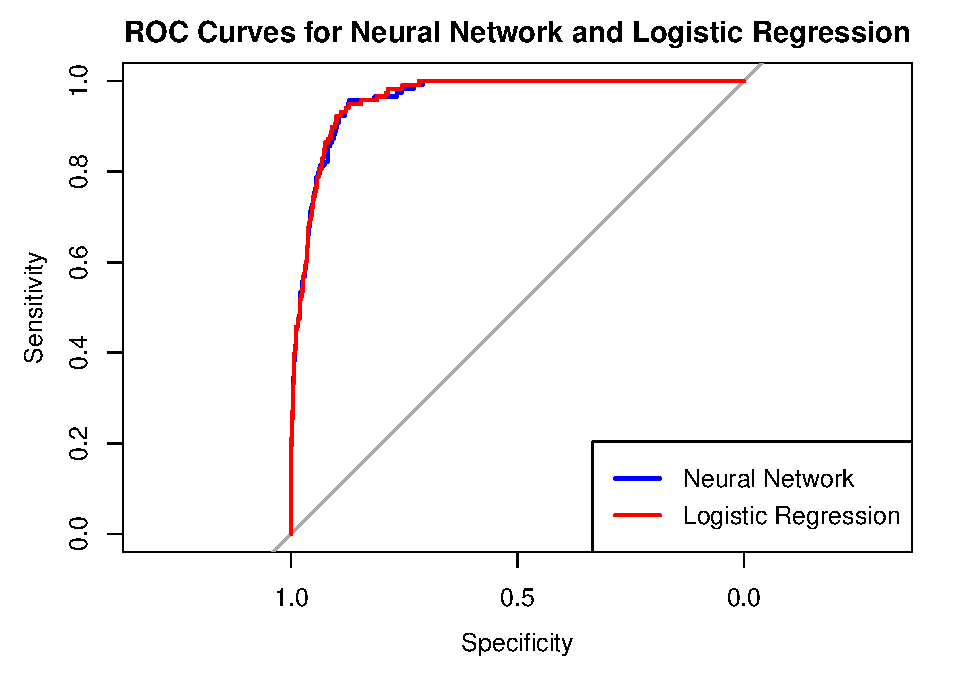
\includegraphics{A2_files/figure-latex/unnamed-chunk-19-1.pdf}

We select 1000 samples as training data and use the remaining ones as
test data.

We then fit a logistic regression model to the training data using all
covariates and determine the misclassification rate and the average
log-likelihood value on the training and test data.

\begin{verbatim}
##      2613      1678      1929      4051       664      1369 
## 0.7890774 0.7872822 0.7666042 0.9905557 0.8772004 0.9584585
\end{verbatim}

\begin{verbatim}
##           7          17          20          29          32          37 
## 0.011710309 0.977713419 0.999999775 0.972453610 0.008824222 0.999858847
\end{verbatim}

\begin{verbatim}
## 
##   0   1 
## 394 606
\end{verbatim}

\begin{verbatim}
## 
##   0   1 
## 304 413
\end{verbatim}

\begin{verbatim}
## 'log Lik.' -205.4046 (df=257)
\end{verbatim}

\begin{verbatim}
## [1] -205.4046
\end{verbatim}

\begin{verbatim}
## [1] -784.7576
\end{verbatim}

\begin{verbatim}
## [1] 0.081
\end{verbatim}

\begin{verbatim}
## [1] 0.2538354
\end{verbatim}

The complexity of this model can be reduced by restricting the
regression coefficients to vary only smoothly over the covariates, i.e.,
regression coefficients for close covariates are similar. To achieve
this, we use splines. We create a 12-dimensional model matrix \(X^*\)
based on natural cubic splines which we use to fit the logistic
regression model instead of the 256-dimensional X. Specifically, we fit
a logistic regression model to the training data using \(X^*\) as model
matrix and determine the misclassification rate and the average
log-likelihood value on the training and test data. The likelihood
function of the (multivariate) Bernoulli distribution is given by
\[\prod_{i=1}^n p^{x_i}(1-p)^{1-x_i}\] Taking the logarithm gives us the
log-lieklihood. \[ \sum_{i=1}^n x_i \log(p)+(1-x_i)\log(1-p) \]

\begin{verbatim}
##      2613      1678      1929      4051       664      1369 
## 0.4505464 0.6646359 0.7403148 0.9347068 0.4867466 0.9834415
\end{verbatim}

\begin{verbatim}
##         7        17        20        29        32        37 
## 0.5750164 0.8453260 0.9546407 0.9299374 0.1447402 0.9743832
\end{verbatim}

\begin{verbatim}
## 
##   0   1 
## 379 621
\end{verbatim}

\begin{verbatim}
## 
##   0   1 
## 283 434
\end{verbatim}

\begin{verbatim}
## 'log Lik.' -398.7008 (df=13)
\end{verbatim}

\begin{verbatim}
## [1] -398.7008
\end{verbatim}

\begin{verbatim}
## [1] -281.076
\end{verbatim}

\begin{verbatim}
## [1] 0.178
\end{verbatim}

\begin{verbatim}
## [1] 0.1659693
\end{verbatim}

We vary the degrees of freedom in the spline basis expansion using 2 to
the power of 1 to 8, i.e., 2,4,8,16,32,64,128 and 256. Again, we
calculate the misclassifiation rate and the mean log-likelihood on the
training and test data for each of the fitted models.

Now we are able to compare the misclassification rates and mean
log-likelihoods based on training and test data sets visually for the
different degrees of freedom.

\includegraphics{A2_files/figure-latex/unnamed-chunk-24-1.pdf}
\includegraphics{A2_files/figure-latex/unnamed-chunk-24-2.pdf}
\includegraphics{A2_files/figure-latex/unnamed-chunk-24-3.pdf}
\includegraphics{A2_files/figure-latex/unnamed-chunk-24-4.pdf} The more
we restrict the regression coefficients to vary only smoothly over the
covariates (lower degrees of freedom), the higher is the
misclassification rate for the training data. Theoretically, higher
smooth avoids overfitting to the training data. But it can also loose
important information. By looking at the misclassification rate of the
test data, we can see that medium levels of degrees of freedom (16-64)
result in the lowest misclassification rate. Low smoot, or in other
words high degrees of freedom, show the expected overfitting. Too much
sommot, low degrees of freedom, seems to loose important information and
hence also increases the misclassification rate on the test data.

On the training data, the log-likelihood worsens with the smooth of the
covariates. Looking at the log-likelihood of the test data we see that
medium levels of degrees of freedom (16-64) are the best choice. They
avoid overfitting and don't loose too much information. Note the very
low log-likelihood due to overiftting for 256 degrees of freedom. On the
other end, with high smooth the loss isn't as high.

\end{document}
